\documentclass[tikz,border=8pt]{standalone}
\usepackage{tikz}
\begin{document}
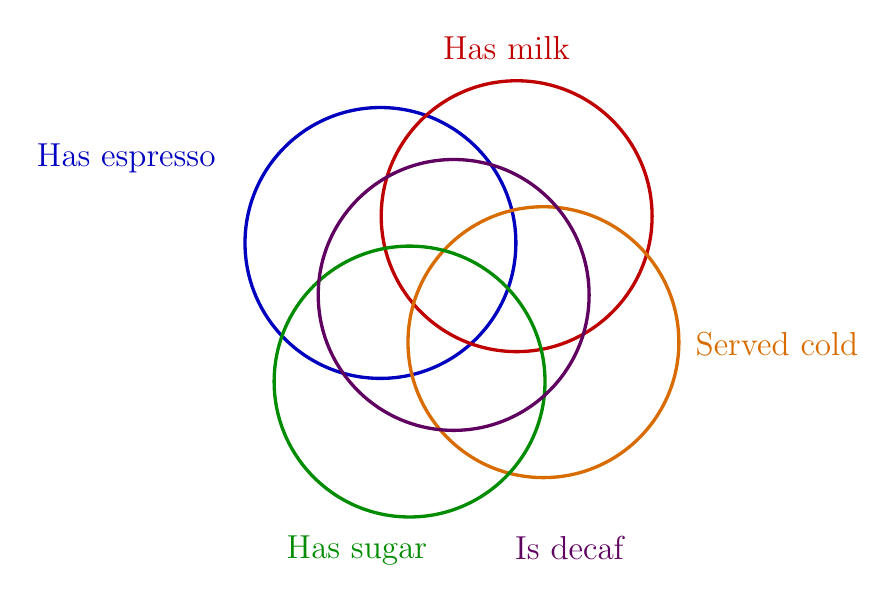
\begin{tikzpicture}[line cap=round]
  % Five generic, pairwise-intersecting circles.  Generic offsets avoid
  % coincident crossings, making every boundary-defined region legible.
  \draw[very thick, blue!75!black]   (-0.95,0.68) circle (1.72);
  \draw[very thick, red!75!black]    (0.78,1.02) circle (1.72);
  \draw[very thick, orange!85!black] (1.12,-0.58) circle (1.72);
  \draw[very thick, green!55!black]  (-0.58,-1.08) circle (1.72);
  \draw[very thick, violet!75!black] (-0.02,0.02) circle (1.72);

  \node[blue!75!black,anchor=east,font=\large] at (-2.92,1.75) {Has espresso};
  \node[red!75!black,anchor=south,font=\large] at (0.65,2.88) {Has milk};
  \node[orange!85!black,anchor=west,font=\large] at (2.93,-0.60) {Served cold};
  \node[green!55!black,anchor=north,font=\large] at (-1.25,-2.92) {Has sugar};
  \node[violet!75!black,anchor=north,font=\large] at (1.45,-2.92) {Is decaf};
\end{tikzpicture}
\end{document}
